%!TEX TS-program = xelatex
\documentclass[12pt, a4paper, oneside]{article}

% Можно вставить разную преамбулу
% пакеты для математики
\usepackage{amsmath,amsfonts,amssymb,amsthm,mathtools}  
\mathtoolsset{showonlyrefs=true}  % Показывать номера только у тех формул, на которые есть \eqref{} в тексте.

\usepackage[british,russian]{babel} % выбор языка для документа
\usepackage[utf8]{inputenc}          % utf8 кодировка

% Основные шрифты 
\usepackage{fontspec}         
\setmainfont{Linux Libertine O}  % задаёт основной шрифт документа

% Математические шрифты 
\usepackage{unicode-math}     
\setmathfont[math-style=upright]{euler.otf} 

\setmathfont[range={\mathbb, \mathop, \heartsuit, \angle, \smile, \varheartsuit}]{Asana-Math.otf}

%%%%%%%%%% Работа с картинками и таблицами %%%%%%%%%%
\usepackage{graphicx} % Для вставки рисунков                
\usepackage{graphics}
\graphicspath{{images/}{pictures/}}   % папки с картинками

\usepackage[figurename=Картинка]{caption}

\usepackage{wrapfig}    % обтекание рисунков и таблиц текстом

\usepackage{booktabs}   % таблицы как в годных книгах
\usepackage{tabularx}   % новые типы колонок
\usepackage{tabulary}   % и ещё новые типы колонок
\usepackage{float}      % возможность позиционировать объекты в нужном месте
\renewcommand{\arraystretch}{1.2}  % больше расстояние между строками


%%%%%%%%%% Графики и рисование %%%%%%%%%%
\usepackage{tikz, pgfplots}  % языки для графики
%\pgfplotsset{compat=1.16}

\usepackage{todonotes} % для вставки в документ заметок о том, что осталось сделать
% \todo{Здесь надо коэффициенты исправить}
% \missingfigure{Здесь будет Последний день Помпеи}
% \listoftodos --- печатает все поставленные \todo'шки

\usepackage{multicol}

%%%%%%%%%% Внешний вид страницы %%%%%%%%%%

\usepackage[paper=a4paper, top=20mm, bottom=15mm,left=20mm,right=15mm]{geometry}
\usepackage{indentfirst}    % установка отступа в первом абзаце главы

\usepackage{setspace}
\setstretch{1.15}  % межстрочный интервал
\setlength{\parskip}{4mm}   % Расстояние между абзацами
% Разные длины в LaTeX: https://en.wikibooks.org/wiki/LaTeX/Lengths

% свешиваем пунктуацию
% теперь знаки пунктуации могут вылезать за правую границу текста, при этом текст выглядит ровнее
\usepackage{microtype}

% \flushbottom                            % Эта команда заставляет LaTeX чуть растягивать строки, чтобы получить идеально прямоугольную страницу
\righthyphenmin=2                       % Разрешение переноса двух и более символов
\widowpenalty=300                     % Небольшое наказание за вдовствующую строку (одна строка абзаца на этой странице, остальное --- на следующей)
\clubpenalty=3000                     % Приличное наказание за сиротствующую строку (омерзительно висящая одинокая строка в начале страницы)
\tolerance=10000     % Ещё какое-то наказание.

% мои цвета https://www.artlebedev.ru/colors/
\definecolor{titleblue}{rgb}{0.2,0.4,0.6} 
\definecolor{blue}{rgb}{0.2,0.4,0.6} 
%\definecolor{red}{rgb}{1,0,0.2} 
\definecolor{green}{rgb}{0, 0.6, 0}
\definecolor{purp}{rgb}{0.4,0,0.8} 

\definecolor{red}{RGB}{213,94,0}
\definecolor{yellow}{RGB}{240,228,66}


% цвета из geogebra 
\definecolor{litebrown}{rgb}{0.6,0.2,0}
\definecolor{darkbrown}{rgb}{0.75,0.75,0.75}

% Гиперссылки
\usepackage{xcolor}   % разные цвета

\usepackage{hyperref}
\hypersetup{
	unicode=true,           % позволяет использовать юникодные символы
	colorlinks=true,       	% true - цветные ссылки
	urlcolor=blue,          % цвет ссылки на url
	linkcolor=black,          % внутренние ссылки
	citecolor=green,        % на библиографию
	breaklinks              % если ссылка не умещается в одну строку, разбивать её на две части?
}

% меняю оформление секций 
\usepackage{titlesec}
\usepackage{sectsty}

% меняю цвет на синий
\sectionfont{\color{titleblue}}
\subsectionfont{\color{titleblue}}

% кружочки у цифр в секциях
\renewcommand{\thesection}{\arabic{section}}

% https://ru.overleaf.com/learn/latex/Sections_and_chapters

% выбрасываю нумерацию страниц и колонтитулы 
%\pagestyle{empty}

% синие круглые бульпоинты в списках itemize 
\usepackage{enumitem}

\definecolor{itemizeblue}{rgb}{0, 0.45, 0.70}

\newcommand*{\MyPoint}{\tikz \draw [baseline, fill=itemizeblue, draw=blue] circle (2.5pt);}
\renewcommand{\labelitemi}{\MyPoint}

\AddEnumerateCounter{\asbuk}{\@asbuk}{\cyrm}
\renewcommand{\theenumi}{\asbuk{enumi}}

% расстояние в списках
\setlist[itemize]{parsep=0.4em,itemsep=0em,topsep=0ex}
\setlist[enumerate]{parsep=0.4em,itemsep=0em,topsep=0ex}

% эпиграфы
\usepackage{epigraph}
\setlength\epigraphwidth{.6\textwidth}
\setlength\epigraphrule{0pt}

%%%%%%%%%% Свои команды %%%%%%%%%%

% Математические операторы первой необходимости:
\DeclareMathOperator{\sgn}{sign}
\DeclareMathOperator*{\argmin}{arg\,min}
\DeclareMathOperator*{\argmax}{arg\,max}
\DeclareMathOperator{\Cov}{Cov}
\DeclareMathOperator{\Var}{Var}
\DeclareMathOperator{\Corr}{Corr}

\DeclareMathOperator{\Pois}{Pois}
\DeclareMathOperator{\Geom}{Geom}
\DeclareMathOperator{\Exp}{Exp}

%\DeclareMathOperator{\E}{\mathbb{E}}
\DeclareMathOperator{\Med}{Med}
\DeclareMathOperator{\Mod}{Mod}
\DeclareMathOperator*{\plim}{plim}

% команды пореже
\newcommand{\const}{\mathrm{const}}  % const прямым начертанием
\newcommand{\iid}{\sim i\,i\,d\,\,}  % ну вы поняли...
\newcommand{\fr}[2]{\ensuremath{^{#1}/_{#2}}}   % особая дробь
\newcommand{\ind}[1]{\mathbbm{1}_{\{#1\}}} % Индикатор события
\newcommand{\dx}[1]{\,\mathrm{d}#1} % для интеграла: маленький отступ и прямая d

% одеваем шапки на частые штуки
\def \hb{\hat{\beta}}
\def \hs{\hat{s}}
\def \hy{\hat{y}}
\def \hY{\hat{Y}}
\def \he{\hat{\varepsilon}}
\def \hVar{\widehat{\Var}}
\def \hCorr{\widehat{\Corr}}
\def \hCov{\widehat{\Cov}}

% Греческие буквы
\def \a{\alpha}
\def \b{\beta}
\def \t{\tau}
\def \dt{\delta}
\def \e{\varepsilon}
\def \ga{\gamma}
\def \kp{\varkappa}
\def \la{\lambda}
\def \sg{\sigma}
\def \tt{\theta}
\def \Dt{\Delta}
\def \La{\Lambda}
\def \Sg{\Sigma}
\def \Tt{\Theta}
\def \Om{\Omega}
\def \om{\omega}

% Готика
\def \mA{\mathcal{A}}
\def \mB{\mathcal{B}}
\def \mC{\mathcal{C}}
\def \mE{\mathcal{E}}
\def \mF{\mathcal{F}}
\def \mH{\mathcal{H}}
\def \mL{\mathcal{L}}
\def \mN{\mathcal{N}}
\def \mU{\mathcal{U}}
\def \mV{\mathcal{V}}
\def \mW{\mathcal{W}}

% Жирные буквы
\def \mbb{\mathbb}
\def \RR{\mbb R}
\def \NN{\mbb N}
\def \ZZ{\mbb Z}
\def \PP{\mbb{P}}
\def \E{\mbb{E}}
\def \QQ{\mbb Q}

\def\F{\ensuremath{\mathcal{F}}} % аналогично!

%%%%%%%%%% Теоремы %%%%%%%%%%
\theoremstyle{plain} % Это стиль по умолчанию.  Есть другие стили.
\newtheorem{theorem}{Теорема}[section]
\newtheorem{proposition}{Утверждение}[section]
\newtheorem{result}{Следствие}[section]

% убирает курсив и что-то еще наверное делает ;)
\theoremstyle{definition}         
\newtheorem*{definition}{Определение}  % нумерация не идёт вообще


%%%%%%%%%% Задачки и решения %%%%%%%%%%
\usepackage{etoolbox}    % логические операторы для своих макросов
\usepackage{environ}
\newtoggle{lecture}

\newcounter{probNum}[section]  % счётчик для упражнений 
\NewEnviron{problem}[1]{%
    \refstepcounter{probNum}% увеличели номер на 1 
    {\noindent \textbf{\large \color{titleblue} Упражнение~\theprobNum~#1}  \\ \\ \BODY}
    {}%
  }

% Окружение, чтобы можно было убирать решения из pdf
\NewEnviron{sol}{%
  \iftoggle{lecture}
    {\noindent \textbf{\large Решение:} \\ \\ \BODY}
    {}%
  }
 
% выделение по тексту важных вещей
\newcommand{\indef}[1]{\textbf{ \color{green} #1}} 

% разные дополнения для картинок
\usetikzlibrary{arrows.meta}
\usepackage{varwidth}

\usepackage[normalem]{ulem}  % для зачекивания текста

% Если переключить в false, все solution исчезнут из pdf
\toggletrue{lecture}
%\togglefalse{lecture}



\title{
\begin{center} 
\includegraphics[width=0.99\textwidth]{logo.png}
\end{center}

Посиделка 7: ЦПТ и ЗБЧ}
\date{ } %\today}

\author{Ульянкин Ппилиф}

\begin{document} % Конец преамбулы, начало файла

\maketitle

\epigraph{Много не мало.}{\textit{(Мой друг Игорь при покупке водки  в баню \newline в расчёте литр на человека)}}

В этой посиделке мы подробно поговорим о теоремах, на которых всё стоит. О законе больших чисел, ЗБЧ и центральной предельной теореме, ЦПТ. В прошлой посиделке было слишком много математики и слишком мало офигительных историй. В этой мы попробуем исправить возникший дисбаланс.


\section{Закон больших чисел в картинках и теоремах}

\indef{Закон больших чисел, ЗБЧ} --- это теорема, которая говорит о том, что среднее арифметическое большого числа похожих случайных величин  «стабилизируется» с ростом их числа. 

Чтобы понять эту мысль, давайте рассмотрим простой пример. Пусть у нас в руках есть игральный кубик. Пусть $X_i$ --- число очков, которое на нём выпало при подбрасывании. Каждая сторона кубика выпадает с вероятностью $\frac{1}{6}.$ Получается, что $\E(X_i) = 3.5.$ 

Давайте будем подкидывать кубик и считать $\bar X$ по мере увеличения количества бросков. По оси $x$ отложим число бросков, по оси $y$ среднее, посчитанное по текущей выборке. По мере увеличения числа бросков, среднее значение всех выпавших исходов будет постепенно приближаться к $3.5$. Именно это и означает, что среднее арифметическое большого числа похожих случайных величин  «стабилизируется» с ростом их числа.

\begin{center} 
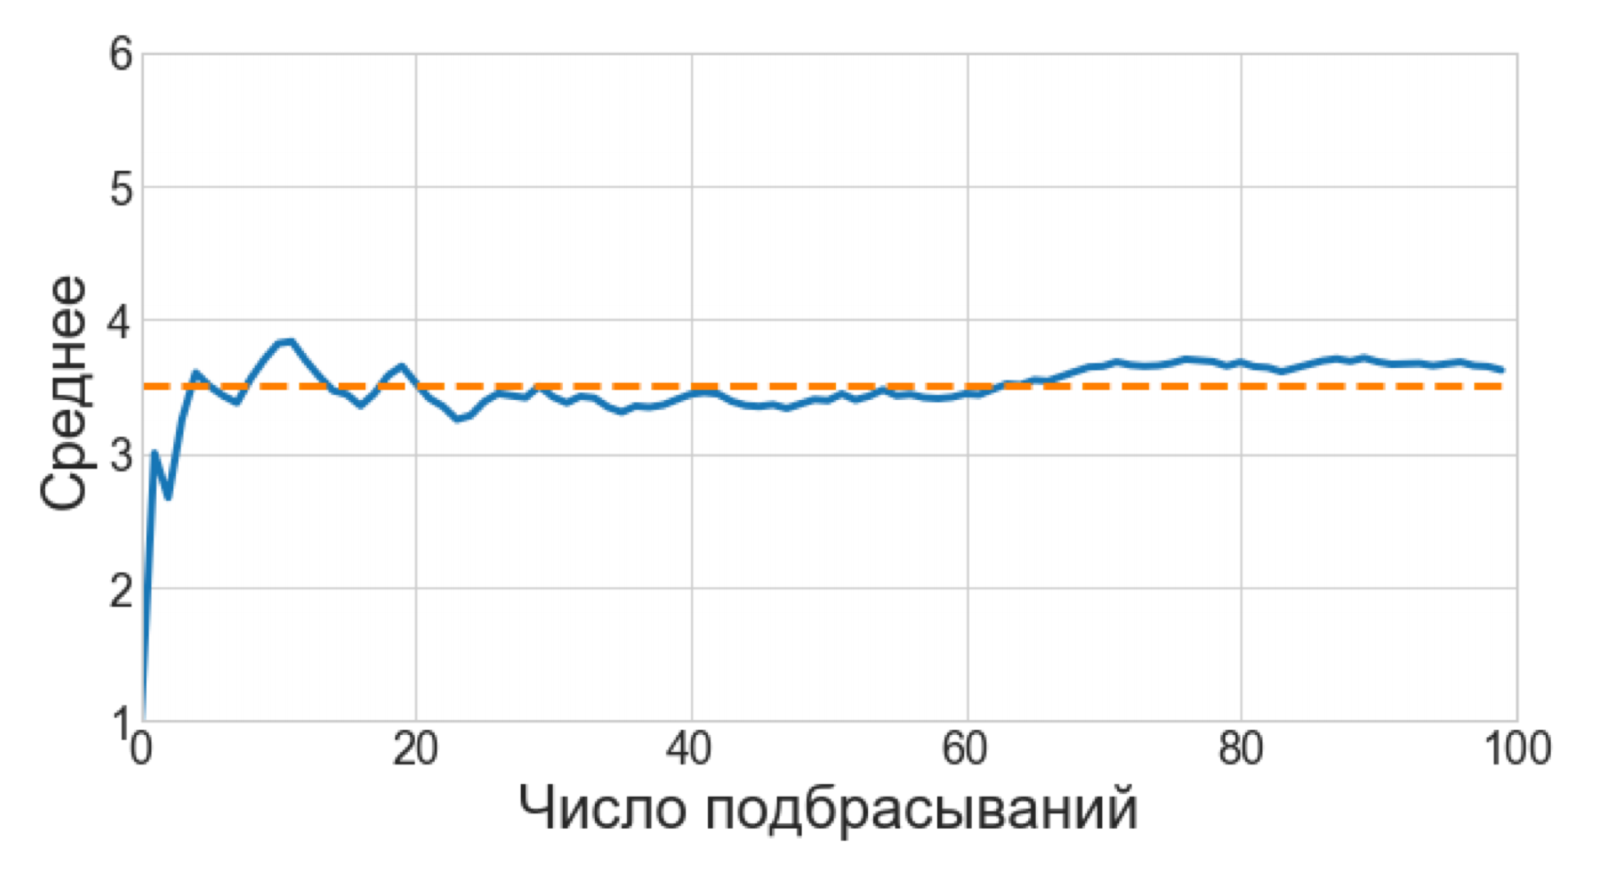
\includegraphics[width=0.8\linewidth]{lln_cube.png}
\end{center} 

Есть много разных теорем, где эта  «стабилизиция» формализуется на математическом языке. Обычно в каждой теореме перечислены условия необходимые для стабилизации, а также конкретный вид стабилизации, то есть сходимость. Мы в этом разделе будем говорить про сходимость по вероятности. Чуть позже мы сформулируем усиленный закон больших чисел, где уже будет фигурировать сходимость почти наверное. 

\begin{theorem}{\textbf{Закон Больших Чисел (Пафнутий Львович Чебышёв)}}

Пусть $X_1, \ldots, X_n$ попарно независимые и одинаково распределённые случайные величины с конечным вторым моментом, $0 < E(X_i^2) < \infty$, тогда

$$
\bar{X}_{n} = \frac{X_1 + \ldots + X_n}{n} \stackrel{p}{\longrightarrow} E(X_1).
$$
\end{theorem}

\begin{proof} 
Нам нужно доказать, что $\forall \varepsilon > 0$ выполняется  $\PP(|\bar{X}_n - \E(X_1)| \ge \varepsilon) \to 0.$ Это определение сходимости по вероятности. Воспользуемся неравенством Чебышёва\footnote{ЗБЧ Чебышёва и неравенство Чебышёва... Совпадение? Не думаю...}

\[
\PP(|\bar{X}_n - \E(X_1)| \ge \varepsilon) \le \frac{\Var(\bar{X}_n)}{\varepsilon^2} = \frac{\Var(X_1)}{n \cdot \varepsilon^2} \to 0 \quad \text{при } n \to \infty.
\]

При подсчёте дисперсии среднего мы воспользовались формулой, которую получили в одной из прошлых посиделок. Конечность второго момента гарантирует нам конечность дисперсии и сходимость к нулю.
\end{proof}

Если у случайные величины независимы, у всех конечные вторые моменты и разные математический ожидания, то заключение теоремы можно переформулировать как 

$$
\bar{X}_{n} = \frac{X_1 + \ldots + X_n}{n} \stackrel{p}{\longrightarrow} \frac{\E(X_1) + \ldots + \E(X_n)}{n}.
$$

Убедитесь сами, что от такой переформулировки в доказательстве ничего не сломается. Мы привели здесь доказательство ЗБЧ Чебышёва ради того, чтобы проиллюстрировать мысль о разных условиях, которые могут накладываться на случайные величины. Например, мы можем легко заменить попарную независимость на попарную некоррелированность. Доказательство от этого не сломается. Более того, ЗБЧ может выполняться для последовательностей из зависимых и разнораспределённых случайных величин.

\begin{theorem}{\textbf{Закон Больших Чисел (Андрей Андреевич Марков)}}

Пусть $X_1, \ldots, X_n$  случайные величины с конечным вторым моментом, $0 < E(X_i^2) < \infty$, при этом 

$$
\frac{\Var(X_1) + \ldots + \Var(X_n)}{n^2} \to 0,
$$

тогда

$$
\bar{X}_{n} = \frac{X_1 + \ldots + X_n}{n} \stackrel{p}{\longrightarrow} \frac{\E(X_1) + \ldots + \E(X_n)}{n}.
$$
\end{theorem}

Теорема Маркова утверждает, что ЗБЧ выполнен, если дисперсия суммы слагаемых растёт с ростом $n$ не очень быстро. Когда слагаемые довольно сильно зависят друг от друга, при раскрытии дисперсии суммы возникают большие ковариации. Из-за этого сходимость часто портится. Что означает здесь слово часто? Можно уточнить условия и сформулировать ещё парочку ЗБЧ, но мы пока что остановимся\footnote{Если хочется копнуть глубже, можно например почитать страницу 191 в книге Гнеденко~\cite{ref:gnedenko}.}.


\section{Чем так хорош ЗБЧ}

Закон больших чисел --- очень классная теорема. Если пытаться упростить её до совсем банального высказывания, то я бы сформулировал ЗБЧ так: «Если у тебя есть страховая фирма, то ты можешь заработать бабла.» 

Впервые ЗБЧ разрешил зарабатывать страховым компаниям деньги в $XVI$ веке. Именно тогда люди впервые начали составлять актуарные таблицы. Это такие таблицы, где указана ожидаемая продолжительность жизни для данного возраста и пола. Люди начали собирать данные о смертности и оценивать вероятность дожития человека до определённого возраста. На этом строились тарифы на страхование. Появление подобных таблиц обязано зарождению в течение 1600-х годов теории вероятности, которая впервые объяснила людям как случайные вещи при достаточно больших масштабах сглаживаются и становятся очень даже предсказуемыми~\cite{zhlobolite}.

В Лондоне $2$ сентября $1666$ года случился пожар. Город горел несколько дней. Когда пожар удалось потушить, один из жителей столицы, Николас Барбон, в прошлом врач, переквалифицировался в застройщика и начал продавать страховки от пожаров. Свою фирму он назвал «Феникс». 

\begin{problem}{(Простая страховка)}
Вероятность того, что на машину во дворе упадёт дерево составляет $0.01$. Страховка в фирме Николаса стоит $10$ рублей в год. В случае, если дерево упало на машину, Николас выплачивает клиенту $2000$ рублей. Какой будет средняя прибыль его компании с одной страховки? 
\end{problem}

\begin{sol}
Пусть случайная величина $X_i$ --- прибыль с одного человека, а $\bar X$ --- средняя прибыль компании. Выпишем распределение $X_i$

\begin{center}
    \begin{tabular}{c|c|c}
    $X_i$          & $10$  & $-1990$ \\ \hline 
    $\PP(X_i = k)$ & $0.99$ & $0.01$ 
    \end{tabular}
\end{center}

По ЗБЧ 

$$
\bar X = \frac{X_1 + \ldots + X_n}{n} \stackrel{p}{\longrightarrow} E(X_i) = 10 \cdot 0.99 - 1990 ⋅ 0.01 = −10.
$$

Получается, что бизнес у Николаса убыточный. 
\end{sol}

Обратите внимание, что мы рассуждаем в предпосылке, что все случайные величины похожи друг на друга. У нас нет выбросов. В жизни они периодически происходят. С лёгкой руки Нассима Талеба такие выбросы, которые всё портят называют \indef{чёрными лебедями.} 

До $1697$ года человечество думало, что лебеди бывают только белыми. Однако голландская экспедиция обнаружила в Западной Австралии популяцию чёрных лебедей. Выражение «чёрный лебедь» используется как метафора того, что весь эмпирический опыт, который был накоплен людьми, может в один момент обесцениться из-за редкого события. Например, тот же Лондонский пожар $1666$ года --- это чёрный лебедь. Огромное количество страховых компаний разорилось из-за подобных больших катастроф. 

Секундочку... Но тогда же это означает, что ЗБЧ не применим к реальной жизни и всё, что я написал в этой главе --- это булщит. На самом деле нет. Когда мы находимся среднестатистическом мире, \indef{в Средиземье,} ЗБЧ и ЦПТ хорошо работают. Как только мы попадаем в мир хвостов распределения, \indef{в Крайнеземье,} начинаются проблемы. Но об этом более подробно мы будем говорить ниже. 

Контрольный вопрос на понимание ЗБЧ. Попробуйте ответить на него сами, а после уже смотрите сноску с верным рассуждением. Пусть мальчики и девочки рождаются равновероятно. В городе есть две больницы: большая и маленькая. В обеих принимают роды. Выяснилось, что в одной из них оценка вероятности появления мальчика составила $0.7$. В какой больнице это скорее всего произошло и почему\footnote{Скорее всего это произошло в маленькой больнице. При малых объёмах выборки вероятность отклониться от $0.5$ больше. Именно об этом говорит нам ЗБЧ.}?

\section{Усиленный закон больших чисел}

На предыдущей посиделке мы выяснили, что сходимости бывают разными. Одной из самых сильных является сходимость почти наверное. Оказывается, что эта сходимость тоже может быть использована для формализации «стабилизиции» последовательности случайных величин.

\begin{theorem}{\textbf{Усиленный Закон Больших Чисел}}

Пусть $X_1, \ldots, X_n$ попарно независимые и одинаково распределённые случайные величины с конечным первым моментом $E(|X_i|) < \infty$, тогда имеет место сходимость:

$$
\frac{X_1 + \ldots + X_n}{n} \overset{a.s.}{\to} E(X_i)
$$
\end{theorem}

Чтобы понять в чём разница с ЗБЧ Чебышёва, надо вспомнить в чём заключается различие между сходимостью по вероятности и сходимостью почти наверное. В обоих ЗБЧ мы говорим, что при больших $n$  среднее $\bar X_n$ скорее всего будет близко к $\E(X_i).$ 

\begin{itemize} 
    \item В случае ЗБЧ Чебышёва мы говорим, что можно сделать вероятность отклонения $\mid X_n - \E(X_i) \mid > \varepsilon$ очень маленькой при достаточно большом $n$. Однако эти отклонения будут происходить. 

    \item В случае усиленного ЗБЧ мы говорим, что отклонения $\mid X_n - \E(X_i) \mid > \varepsilon$ почти наверное не произойдёт. Неравенство $\mid X_n - \E(X_i) \mid  \le \varepsilon$ при больших $n$ будет выполняться с вероятностью равной единице. 
\end{itemize} 

Мы оставим этот ЗБЧ без доказательства \footnote{Оно выглядит громоздко. Можно найти пример в N. Etemadi, An Elementary Proof of the Strong Law of large numbers. Z. Wahrsch. Verw. Gebiete, 55(1981):119--122, 1981. \newline Проще доказать ЗБЧ, если предположить существование четвёртого момента, такое доказательство смотри в Sheldon Ross, A First Course in Probability. Printice Hall, Upper Saddle River, New Jersey 07458, Eighth Edition, 2010}. 


\section{Центральная предельная теорема}

\indef{Центральная предельная теорема, ЦПТ,} говорит, что сумма довольно большого числа случайных величин имеет в пределе распределение близкое к нормальному, если среди этих случайных величин нет каких-то выбросов, аномалий, и они в целом друг на друга очень сильно похожи.

Снова давайте посмотрим на игральные кубики. Когда мы подкидываем одну игральную кость, она равновероятно может принять значение $1, 2, 3, 4, 5, 6$. Если мы подкинем игральную кость два раза, то сумма уже будет принимать значение с разными вероятностями.  Значение $2$ эта сумма примет с более низкой вероятностью, чем значение $6$. Двойку можно получить только как сумму из двух единичек, а шестёрку можно получить кучей способов. Как два и четыре, три и три, один и пять.  При этом значение $12$ тоже можно получить только одним способом. Распределение суммы будет выглядеть как треугольник. 

\begin{center} 
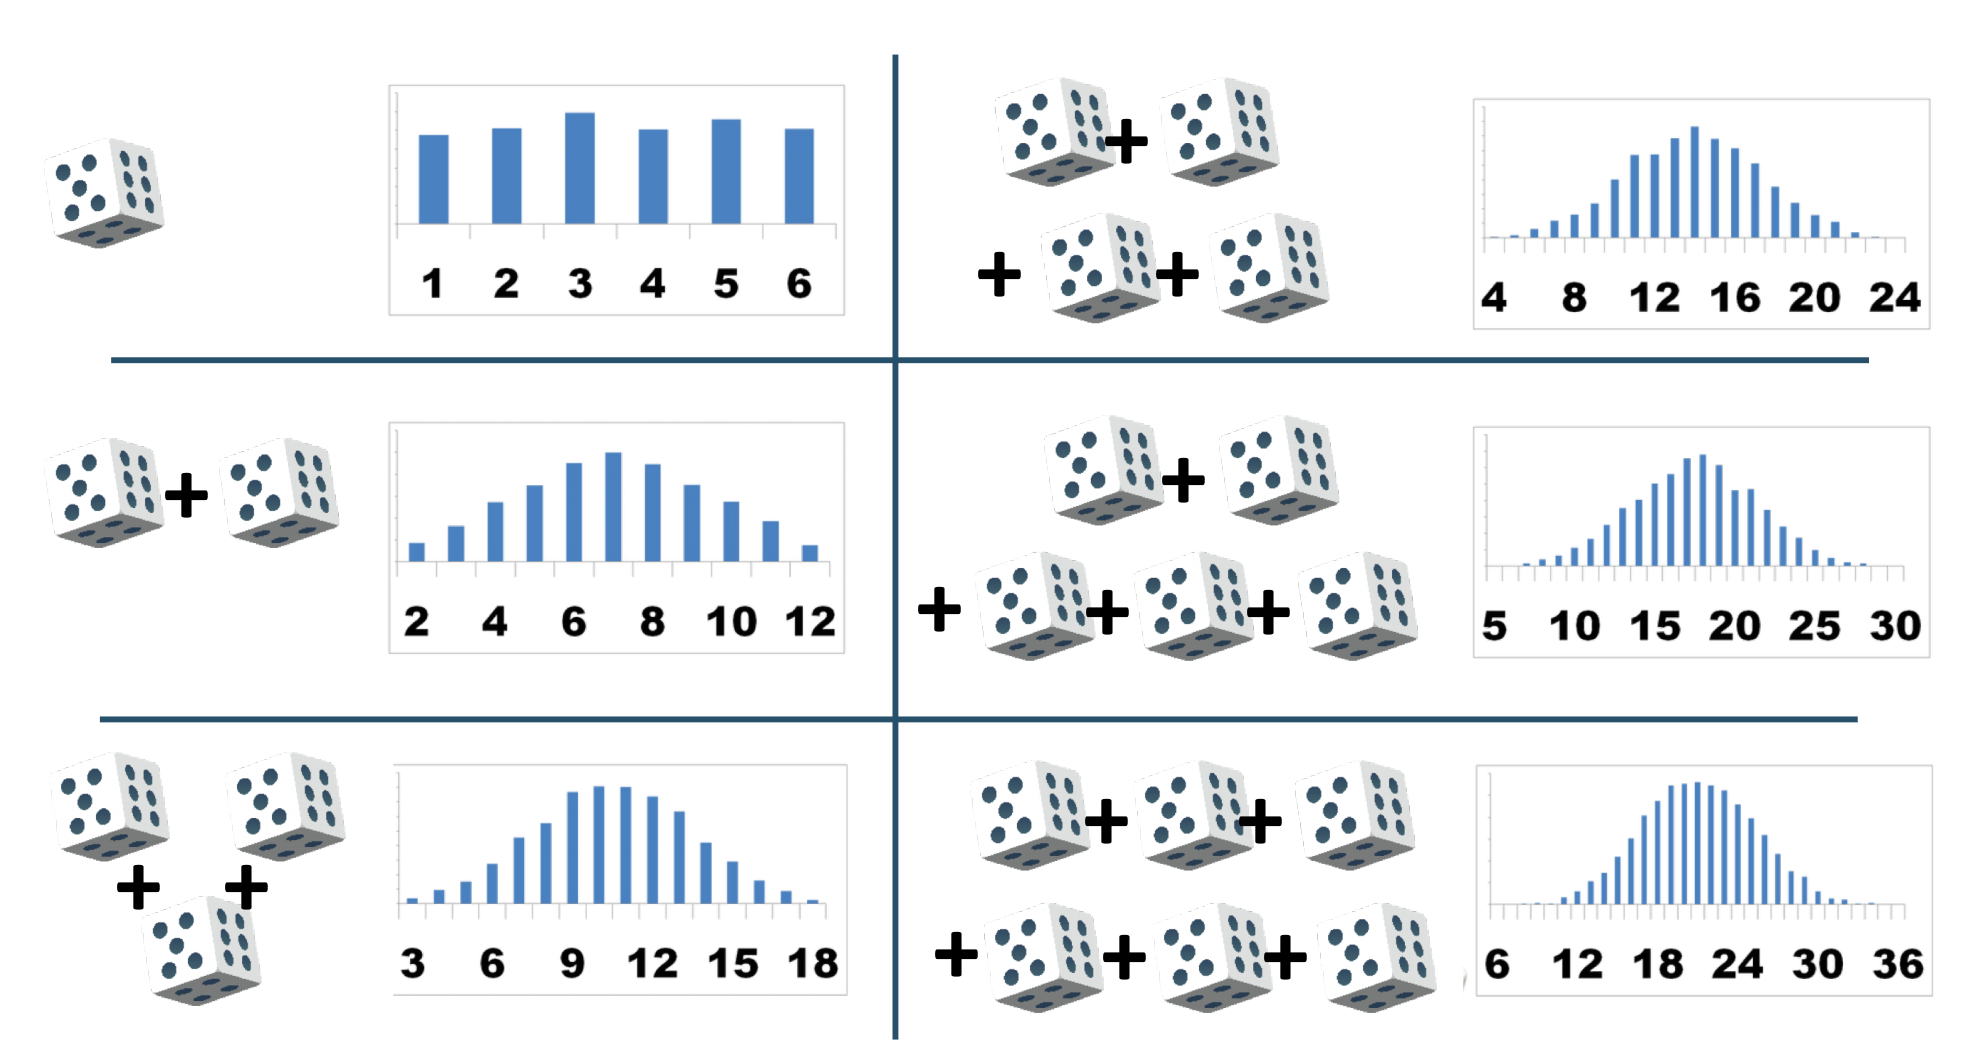
\includegraphics[width=0.95\linewidth]{clt_cube.png}
\end{center} 

Если мы подкинем $3$ игральные кости, то распределение станет еще более куполообразным, если подкинем $4$, распределение станет еще куполообразнее. Чем больше случайных величин мы будем суммировать, тем ближе к нормальному будет итоговое распределение. Именно об этом и говорит нам ЦПТ. На практике мы часто считаем средние. Именно в этом месте ЦПТ оказывается для нас хорошим помощником, на базе которого можно сделать вывод о том, насколько разнообразные значения это среднее может принимать. По аналогии с ЗБЧ есть много разных формулировок ЦПТ с разными предпосылками. 

\begin{theorem}{\textbf{Центральная Предельная Теорема (Прокопий Петрович Ляпунов)}}

Пусть $X_1, \ldots, X_n$ попарно независимые и одинаково распределённые случайные величины с конечным вторым моментом, $E(X_i^2) < \infty$, тогда при $n \to \infty$ имеет место сходимость по распределению: 

\[\sqrt{n} \cdot [\bar X - \E(X_i)]  \overset{d}{\to} N \left(0, \Var(X_i)\right)\]

Этот же факт можно переписать немного иначе

\[\sqrt{n} \cdot \frac{\bar{X} - \E(X_i)}{\sqrt{\Var(X_i)}}  \overset{d}{\to} N \left(0, 1\right)\]

или даже как

$$
\bar{X} \overset{\text{\textit{asy}}}{\sim} N \left(\E(X_i), \frac{\Var(X_i)}{n} \right).
$$

Подпись \textit{asy} означает, что таким распределением мы можем приблизть распределение среднего при большом размере выборки $n$.
\end{theorem}

Если говорить простым языком, то при определённых условиях сумма достаточно большого числа случайных величин имеет распределение близкое к нормальному. Есть очень большое количество формулировок ЦПТ с разными условиями и скоростями сходимости. \indef{Глобально в этих условиях главное, чтобы случайные величины были похожи и не было такого, что одна резко выделяется на фоне остальных.} 

Посмотрим еще на один пример. Предположим, что случайная величина $X$ --- время прихода Ратибора на первую пару. Если Ратибор опоздал на пару, то $X$ принимает значение того времени, на какое он опоздал. Если он пришел заранее, то случайная величина $X$ принимает отрицательное значение. Это время складывается из большого количества разных мелких случайностей. 

Сегодня утром на Ратибора прыгнул его кот, Батый. Из-за этого пришлось встать пораньше. У нас появилась случайная величина $X_1,$ которая войдёт в нашу итоговую случайную величину $X.$ Дальше Ратибор решил поесть хлопушки с тёплым молоком, но оно убежало. Пришлось убираться. Возникла задержка на $X_2.$  Дальше, автобус приехал пораньше, Ратибору повезло, но, к сожалению, по ходу своего маршрута он встал в гигантскую пробку, и из-за этого задержался ещё сильнее. 

В итоге время прихода Ратибора на пару складывается из огромного количества случайностей, которые состыкуются между собой. И если ни одна из этих случайностей не выделяется резко на фоне всех остальных, то время прихода, $X$ хорошо аппроксимируется нормальным распределением. 

Если кот Батый прыгает на Ратибора очень-очень рано, и Ратибор едет на пару, не засыпая по второму кругу, нормальность сломается. Хвост, в котором Ратибор приходит заранее, будет более толстым. Из-за кота приходы заранее будут более вероятными, чем опоздания.

\begin{problem}{(Резервы для страховки)}
Портфель страховой компании состоит из $1000$ договоров, заключенных $1$
января и действующих в течение года. При наступлении страхового случая по каждому из договоров компания обязуется выплатить $1500$ рублей.

Вероятность наступления страхового события по каждому из договоров предполагается равной $0.05$ и не зависящей от наступления страховых событий по другим контрактам. Каков должен быть совокупный размер резерва страховой компании для того, чтобы с вероятностью $0.95$ она могла бы удовлетворить требования, возникающие по указанным договорам?
\end{problem}

\begin{sol}
Пусть случайная величина $X_i$ принимает значение $1$, если для $i-$го клиента наступил страховой случай. Тогда общее число страховых случаев 

\[
Y = \sum_{i=1}^n X_i \sim Bin(n=1000, p=0.05).
\]

Пусть $S$ --- размет резерва. Тогда условие на него можно записать в виде $\PP(1500 Y \leq S) = 0.95$. Решать это уравнение, используя биномиальное распределение, довольно сложно. Учитывая, что у нас много клиентов и возникновение страховых случаев распределено одинаково, мы можем воспользоваться ЦПТ

\[
\frac{1}{n} \sum_{i=1}^n X_i \overset{\text{\textit{asy}}}{\sim} \mN \left(\E(X_i), \frac{\Var(X_i)}{n} \right).
\] 

Значком $asy$ над тильдой обычно подчёркивают, что речь идёт о том, что мы аппроксимируем распределение с помощью нормального, то есть все вычисления, которые мы будем делать, верны при большом $n$. Посчитаем характеристики распределения 

\[
\E(X_i) = 0.05, \quad \Var(X_i) = 0.05 \cdot 0.95.
\]

Выходит, что \[Y \overset{\text{\textit{asy}}}{\sim} \mN(1000 \cdot 0.05, 1000 \cdot 0.05 \cdot 0.95).\] 

Чтобы найти требуемую вероятность, вычтем из $Y$ математическое ожидание и поделим на стандартное отклонение

\[
\PP(1500 Y \leq S) = \PP\left(Y \leq \frac{S}{1500} \right) = \PP\left(\frac{Y - 50}{\sqrt{1000 \cdot 0.05 \cdot 0.95}} \leq \frac{\frac{S}{1500}-50}{\sqrt{1000 \cdot 0.05 \cdot 0.95}} \right) = 0.95.
\]

Воспользуемся тем, что $95\%$ квантиль стандартного нормального распределения примерно равен $1.65$
\[
\frac{\frac{S}{1500}-50}{\sqrt{1000 \cdot 0.05 \cdot 0.95}} \approx 1.65 \Rightarrow S \approx 92058.
\]
\end{sol}


\begin{problem}{(Простая страховка)}
Вероятность того, что на машину во дворе упадёт дерево составляет $0.01$. Страховка в фирме Николаса стоит $10$ рублей в год. В случае, если дерево упало на машину, Николас выплачивает клиенту $2000$ рублей. 
У Николаса есть $n$ клиентов. Как распределена средняя прибыль компании? Какова вероятность того, что компания получит положительную среднюю прибыль? Что происходит при $n \to \infty$?
\end{problem}

\begin{sol}
Речь идёт о среднем. Выплаты всем клиентам имеют одинаковое распределение, а значит мы можем воспользоваться ЦПТ. В предыдущих посиделках мы уже находили математическое ожидание и дисперсию для среднего, а значит можем смело записать, что 

\[
\bar{X} \overset{\text{\textit{asy}}}{\sim} \mN \left(\E(X_i), \frac{\Var(X_i)}{n} \right).
\] 

Выходит, что 

\[
\bar{X} \overset{\text{\textit{asy}}}{\sim} \mN \left(-10, \frac{39600}{n} \right).
\] 

Найдём вероятность того, что прибыль окажется положительной

\[
\PP \left(\bar{X} > 0 \right) = \PP \left(\frac{\bar{X} - (-10)}{\sqrt{39600/n}} > \frac{10}{\sqrt{39600/n}} \right) \approx 1 - \Phi\left( \sqrt{n} \cdot \frac{10}{199} \right) = 1 - \Phi ( 0.05 \cdot \sqrt{n}).
\]

Если $n=100$ вероятность положительной прибыли оказывается $0.31$. При $n=1000$ вероятность положительной прибыли уже $0.06$, при $n=5000$ она уже около нуля. Когда у Николоса мало клиентов, положительная прибыль может получиться довольно случайно. Когда клиентов становится много, дисперсия убывает и средняя прибыль стабилизируется в районе $-10$. Асимптотика работает против его страховой фирмы. 
\end{sol}

Обратите внимание, что предельные теоремы бывают разными. Например, для приближения биномиального распределения часто используют распределение Пуассона. Но про это мы пока что говорить не будем. 


\section{Когда наступает асимптотика} 

На самом деле это всё только приближение. Для каждого конкретного $n$ распределение отличается от нормального. Сходимость к нормальному распределению довольно сильно зависит от конкретного семейства распределений, с которым мы работаем. Например, для равномерного распределения сходимость наступает довольно быстро.

\todo[inline]{Пример}

сюда про сумму из 5 равномерных и доску гальтона + неравенство Бэри-Эссена









\section{Самое опасное уравнение}

Незнание того, как именно размер выборки влияет на статистические различия, создавало хаос на протяжении тысячелетия. В людском эпосе накопилось довольно много офигительных историй про это. В этом разделе я перескажу вам несколько таких историй из статьи «The Most Dangerous Equation»~\cite{ref:zmde}. 

Что из себя может представлять опасное уравнение? Опасность может представлять два вида формул: те, которые вы знаете и те, которые вы не знаете. Первая категория уравнений может открывать для людей двери, за которыми находится смертельная опасность. Например, уравнение Эйнштейна открыло человечеству дорогу к атомной бомбе. 

Однако нам интереснее другие уравнения. Уравнения, которые раскрывают свою опасность не тогда, когда мы знаем о них, а скорее тогда, когда мы их не знаем. Находясь под рукой, эти уравнения позволяют нам ясно понимать как работает природа. Незнание оставляет нас в опасном неведении. 

\subsection{Испытание Пикса}

В $1150$ году было решено, что король Англии не может чеканить деньги и присваивать им любую ценность по своему выбору. Вместо этого ценность монеты должна была быть внутренней, основанной на том, сколько в её составе драгоценных материалов. Были установлены стандарты, сколько в какой монете должно быть золота. Чтобы проверить соответствует ли новая партия монет стандартам, проводили испытание Пикса. Пикс (pyx) --- это деревянный ящик, в котором находились стандартные монеты с правильным содержанием золота. Проверками занималась независимая организация, Монетный двор. Она состояла из баронов короля.

Монетный двор прекрасно понимал, что нельзя отчеканить абсолютно точную монету. Поэтому брали выборку новых монет, например сотню, и сравнивали её со стандартом. Надо было, чтобы эта сотня соответствовала заявленному уровню плюс минус некоторая погрешность. В качестве погрешности выбрали $\frac{1}{400}$ веса. Вес монет тогда измеряли в гранах (grain)\footnote{Единица измерения массы, основанная на весе ячменного зерна.}. Одна монета должна была весить $128$ гран. Получается, что суммарный вес сотни монет должен был оказаться в диапазоне $12800 \pm 32$ гран\footnote{У автора почему-то $ \tfrac{1}{400}\cdot 128 = 0.28.$ Видимо, он у баронов в доле. За поимку этого бага большое спасибо Борису Демешеву.}. 

Если мы пробили левую границу, надо казнить чеканщика за воровство. Если мы пробили правую границу, надо брать всю партию и переделывать, так как потрачено слишком много золота. Проблема в том, что интервал для суммы оказывался слишком широким, так как Монетный двор предполагал, что погрешность изменяется пропорционально числу монет. О том, что погрешность пропорциональна квадратному корню из числа монет, станет известно только через $600$ лет благодаря Муавру.

Из-за слишком широкого интервала и страха казни, перекос был в сторону слишком тяжёлых монет. Скорее всего, были люди, которые чувствовали этот косяк в методологии Монетного двора и использовали его. Надо было просто брать из свежей партии монет самые тяжёлые, переплавлять их и навариваться на их переплавке в типовые.  

Попробуйте поразмышлять над решением следующей задачи, чтобы разобраться в ошибке Лондонского Монетного двора. 

\begin{problem}{(Нужно больше золота)}
Древние короли Вестероса постановили, что каждая новая партия золотых монет должна сравниваться по весу со стандартом. Одна стандартная монета весит $128$ гран. Десница короля лично извлекает из каждой новой партии монет $100$ случайных и измеряет их вес. Вес каждой монеты не должен отличаться от $128$ больше, чем на $\frac{1}{400}$ веса.

Если вес монет лежит в диапазоне $12800 \pm 100 \cdot 0.32$ грана, партия монет поступает в казну. Если вес слишком маленький, Мастера над Монетой казнят. Если вес слишком большой, партию отправляют на повторную переплавку. Будем считать, что стандартное отклонение у способа чеканки, принятого в королевстве, действительно составляет $0.32$. 

\begin{enumerate} 
    \item В каком диапазоне с вероятностью $0.95$ находится суммарный вес $100$ монет? В каком диапазоне он находится с вероятностью $0.997$? Совпадает ли с каким-то из этих двух интервалов методология короля?
    
    \item Десница решил использовать вместо $100$ монет $200$. Будет ли $99\%$ доверительный интервал совпадать с методологией Монетного двора? 

    \item Мастер над Монетой опасается казни. Сколько лишнего золота ему нужно добавлять в монету, чтобы его не казнили с вероятностью $0.95$?
    
    \item С какой вероятностью в условиях предыдущего пункта партия будет уходить на переплавку? Как часто это будет происходить? 
\end{enumerate} 
\end{problem}

% \begin{sol}
% \todo[inline]{Написать или нет...}
% \end{sol}


\subsection{Насколько хорошо жить в деревне?} 

Центральная предельная теорема и Закон Больших чисел справедливы только при бесконечно больших $n$. При просто больших $n$ они работают <<приближённо>>. Это замечательные теоремы, правда у них есть своя довольно жёсткая сфера применимости. 


\section{Средеземье, Крайнеземье и тяжёлые хвосты}

Грубо говоря, все методы в статистике можно поделить на две части. Первая часть методов работает с средней частью распределения. Я пафосно буду называть эту часть Средиземьем. Нормальные люди в нормальных источниках так её не называют. В Средиземье у нас работает и центральная предельная теорема, и закон больших чисел. Мы можем успешно их применять на практике. 

Вторая часть методов работает с хвостами распределений, с Крайнеземьем. Основная проблема, связанная с хвостами заключается в том, что они иногда оказываются \indef{тяжёлыми.} На картинке ниже хвосты красного распределения тяжелее хвостов синего распределения. Под ними сосредоточено больше вероятностной массы. Это означает, что редкие событие для красного распределения происходят чаще, чем для синего.

\begin{center} 
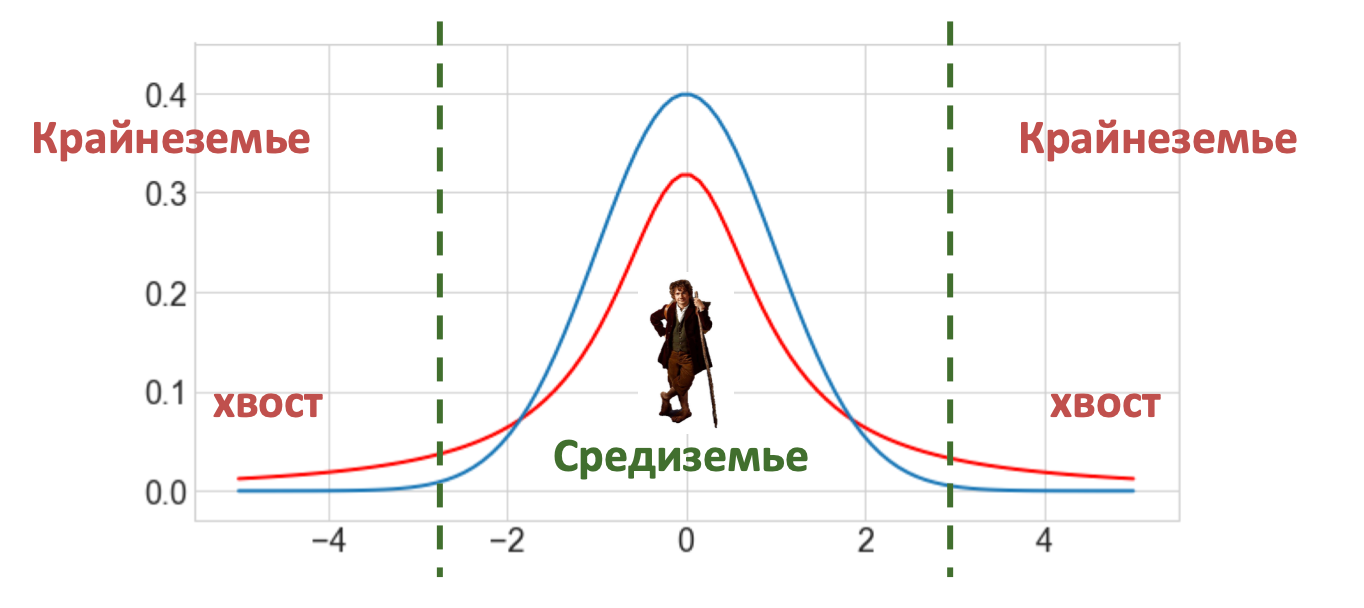
\includegraphics[width=0.8\linewidth]{tails.png}
\end{center} 

По сравнению с серединой распределения хвосты очень тонкие. Статистики по событиям из них к нам в выборки приходит довольно мало. Из-за этого хвосты часто недооценивают, а вероятность событий из них занижают. 

Событий из хвостов обычно никто не ждёт, а когда они наступают, люди довольно сильно от этого страдают. Как уже отмечалось, с лёгкой руки Нассима Талеба, такие события называют \indef{чёрными лебедями.} Отсутствие статистики приводит к недооценке. Её надо как-то скорректировать. Для подобной коррекции придумано довольно много методов. Подробный разговор о статистике Крайнеземья мы отложим на будущие посиделки. Сейчас мы сконцентрируемся на том, что происходит в Средиземье и обсудим мощь средних. Но перед этим давайте обсудим две офигительные истории про хвосты. 

\subsection{Финансовые рынки и азартные игры} 

Забавно, что изначально теорию вероятности развивали аристократы, которых заинтересовало то, как работают азартные игры\footnote{Иван, который вкладывается в крипту на всю котлету не дурак, а потенциальный отец-основатель совершенно новой ветви математики.}. Кардано и Бернулли размышляли о том как выпадают Кости и попутно строили основы теории вероятностей~\cite{ref:gnedenko}.

В $XX$ веке особо ничего не поменялось. Например, в $1961$ Эд Торп и Клод Шеннон вместе пытались разработать выигрышную стратегию для игры в рулетку. В ходе опытов они создали первый портативный компьютер. Устройство размером с пачку сигарет клался в ботинок. В первый раз он нажимал пальцем ноги на кнопку, когда рулетку запускали. Второй раз, когда колесо делало один оборот. Компьютер вычислял будущее положение шарика и посылал игроку радиосигнал. У него под одеждой был радиоприёмник, от которого шел провод к динамику в ухе. Система работала, но с компьютером постоянно происходили проблемы. Динамик вываливался из уха, а провода рвались. 

Торп активно думал над тем, как выиграть в блэкджек c $1958$ года. Во время игры состав колоды меняется. Какие-то карты выбывают, какие-то остаются. Это влияет на преимущество игрока или казино. Чтобы вывести выгодные для игрока закономерности, надо перебрать миллионы карточных комбинаций. Торпп сделал это на университетском компьютере и выяснил, что чем больше в колоде остается девяток, десяток (это также дамы, короли и валеты) и тузов, тем лучше для игрока. Он разработал несколько стратегий подсчёта карт. В 1960 году наконец вывел оптимальную выигрышную стратегию — подсчёт десяток. Тур по разным казино показал, что стратегия работала. Закон больших чисел в очередной раз позволил зарабатывать деньги. Он написал об этом книгу <<Обыграй диллера>>~\cite{ref:torp}.  

Торп стал персоной нон грата для многих казино. Чтобы местные воротилы не избили его и не отдали выигрыш, Торп маскировался и переодевался. Владельцы казино пытались подмешивать ему в напитки наркотики. Торпу стало страшно за свою жизнь. Он решил проверить дадут ли его методы выигрыша в азартных играх преимущество на финансовых рынках. В итоге он основал несколько хэдж-фондов и стал миллиардером. Фактически Торп стал отцом-основателем количественных финансов. В течение $90-$х у него появилось огромное число последователей, а сам мир финансов очень сильно изменился. В каждом крупном банке появилась группа, торговавшая с помощью математических алгоритмов. В книге <<Кванты>> Скотта Паттерсона красочно описывается как именно это происходило и  как привело к мировому финансовому кризису $2008$ года~\cite{ref:quant}. 


Одной из причин обвала было то, что математические модели очень сильно недооценивали хвосты распределений. В моделях активно использовалась ЦПТ и нормальные распределения. В Средиземье это было бы позволительно. Например, если вы измеряете рост $1000$ человек, вряд ли $1001-$е измерение повлияет на среднее существенным образом. В мире финансов даже маленькое колебание цены может изменить всё. Если мы смотрим на распределение доходов, оно в среднем нормальное. Но если в выборку попадает Билл Гейтс, распределение неожиданно изменится. 

С ценами на рынках такая же история. Скачки могут быть очень сильными. Рынки имеют тенденцию к более резким движениям. Например, во время кризиса $2008-$го цены в течение дня могли изменяться на $25$ стандартных отклонений. В течение дня происходили события, которые не должны были происходить с точки зрения моделей никогда~\cite{ref:quant}. 


После кризиса $2008$ года методы работы с тяжёлыми хвостами стали широко распространены в финансах. Нассим Талеб, кстати говоря, сильно приложил к этому руку. Ещё до кризиса он активно критиковал используемые трейдерами модели вместе с Бенуа Мандельбротом. Свою точку зрения Талеб активно подтверждал делом.

Например, во время обвала в Чёрный понедельник $19$ октября $1987$ года, Талеб стал богаче на $40$ миллионов долларов. Он менял инвестиционные компании как перчатки и параллельно получал докторскую степень. В $1999$ году он начал вести курс по финансам в Нью-Йоркском университете и одновременно запустил свой собственный хедж-фонд.  В $2008$ году  фонд Universa Investments, связанный с Талебом, заработал $150\%$ на ставках, что рынок намного волатильнее, чем считают все остальные.  

Методы для работы с тяжёлыми хвостами сегодня довольно широко распространены в финансах. Именно в хвостах распределений находятся самые крупные финансовые потери. Для того, чтобы знать, сколько денег мы можем потерять при самом неблагоприятном исходе обычно вычисляют такую меру риска как \indef{VaR — Value at risk.}

На самом деле это просто-напросто какой-то квантиль, например, уровня $5 \%.$ Ниже него находится $5\%$ вероятностной массы распределения. Если речь идёт о доходности ценной бумаги, то левее этого квантиля находятся наши потери. Получается, что именно такую величину либо более экстремальную мы потеряем в $5\%$ случаев. Понятное дело, что если мы хотим получить хорошую оценку на самые неблагоприятные исходы, то мы должны моделировать хвост довольно хорошо.

К счастью кризисы происходят редко. Каждый из них уникален по-своему. Человечество идёт вперёд. Каждые $10$ лет во временных рядах происходит структурный сдвиг. Из-за этого у нас есть довольно мало статистики о том, что происходит в хвосте распределения с доходностью. Для того, чтобы получить адекватную оценку для $VaR,$ приходится привлекать довольно специфические методы. 


\subsection{Ребята, давайте жить дружно}

В $2011$ году у Стивена Пинкера из Гарварда вышла книга <<Лучшее в нас>> про исследования, которые показывают, что в мире стало меньше насилия~\cite{ref:pinker}.  Мы живём в самое прекрасное и мирное время в истории. Стало меньше войн, массовых казней, геноцидов вообще нет. Ядерное оружие всех сдерживает от мировой войны. Работорговля и жертвоприношения сократились, бытового насилия стало меньше. 

Проблема в том, что этот тезис Пинкер подтверждает только графиками и не делает каких-то серьёзных расчётов. Довольно серьёзную критику идей Пинкера провёл Нассим Талеб, который сначала сравнил теорию о сокращении количества войн и насилия с теорией растущего без обвалов фондового рынка, а потом написал целую статью с проверкой гипоптезы о том, что насилие действительно идёт на спад~\cite{ref:taleb}. 

Талеб с соавторами собрал данные из самых современных источников, обработали перекосы в них, убедились, что для войн, правый хвост очень тяжёлый и использовали для его моделирования соответствующие методы. Оказалось, что пока что никакого тренда на снижение насилия пока что нет. 

Если говорить о будущем, то вероятность большой войны очень низка. Мы оказываемся на территории Крайнеземья. Статистика Пинкера показывает, что крупная война с максимальным числом погибших случается примерно раз в 100 лет. После Второй мировой войны ещё сто лет не прошло, поэтому некорректно говорить о смене тренда. Пинкер в ответ отвечает, что в $1945$ произошёл структурный сдвиг, однако расчёты, которые могли бы это подтвердить, сделать пока нельзя. Слишком мало данных накопилось после Второй мировой войны. Кто из учёных прав непонятно. 

Важно следить, с какой именно зоной распределения мы работаем, иначе можно получить некорректные выводы и оценки. Ну либо устроить новую Великую Рецессию, как в $2008$~\cite{ref:quants}. 

\subsection{ЕГЭ в Польше}

На Крайнеземье немного посмотрели. Теперь давайте теперь посмотрим на пару примеров ситуаций, когда мы оказываемся в Средиземье. На Reddit есть трэд, где обсуждают распределение результов Польского ЕГЭ\footnote{\url{https://www.reddit.com/r/poland/comments/ber86s/distribution_of_final_exam_scores_in_poland/}}. Оно изображено на картинке ниже. Как думаете, что странного есть на этой гистограмме?

\begin{center} 
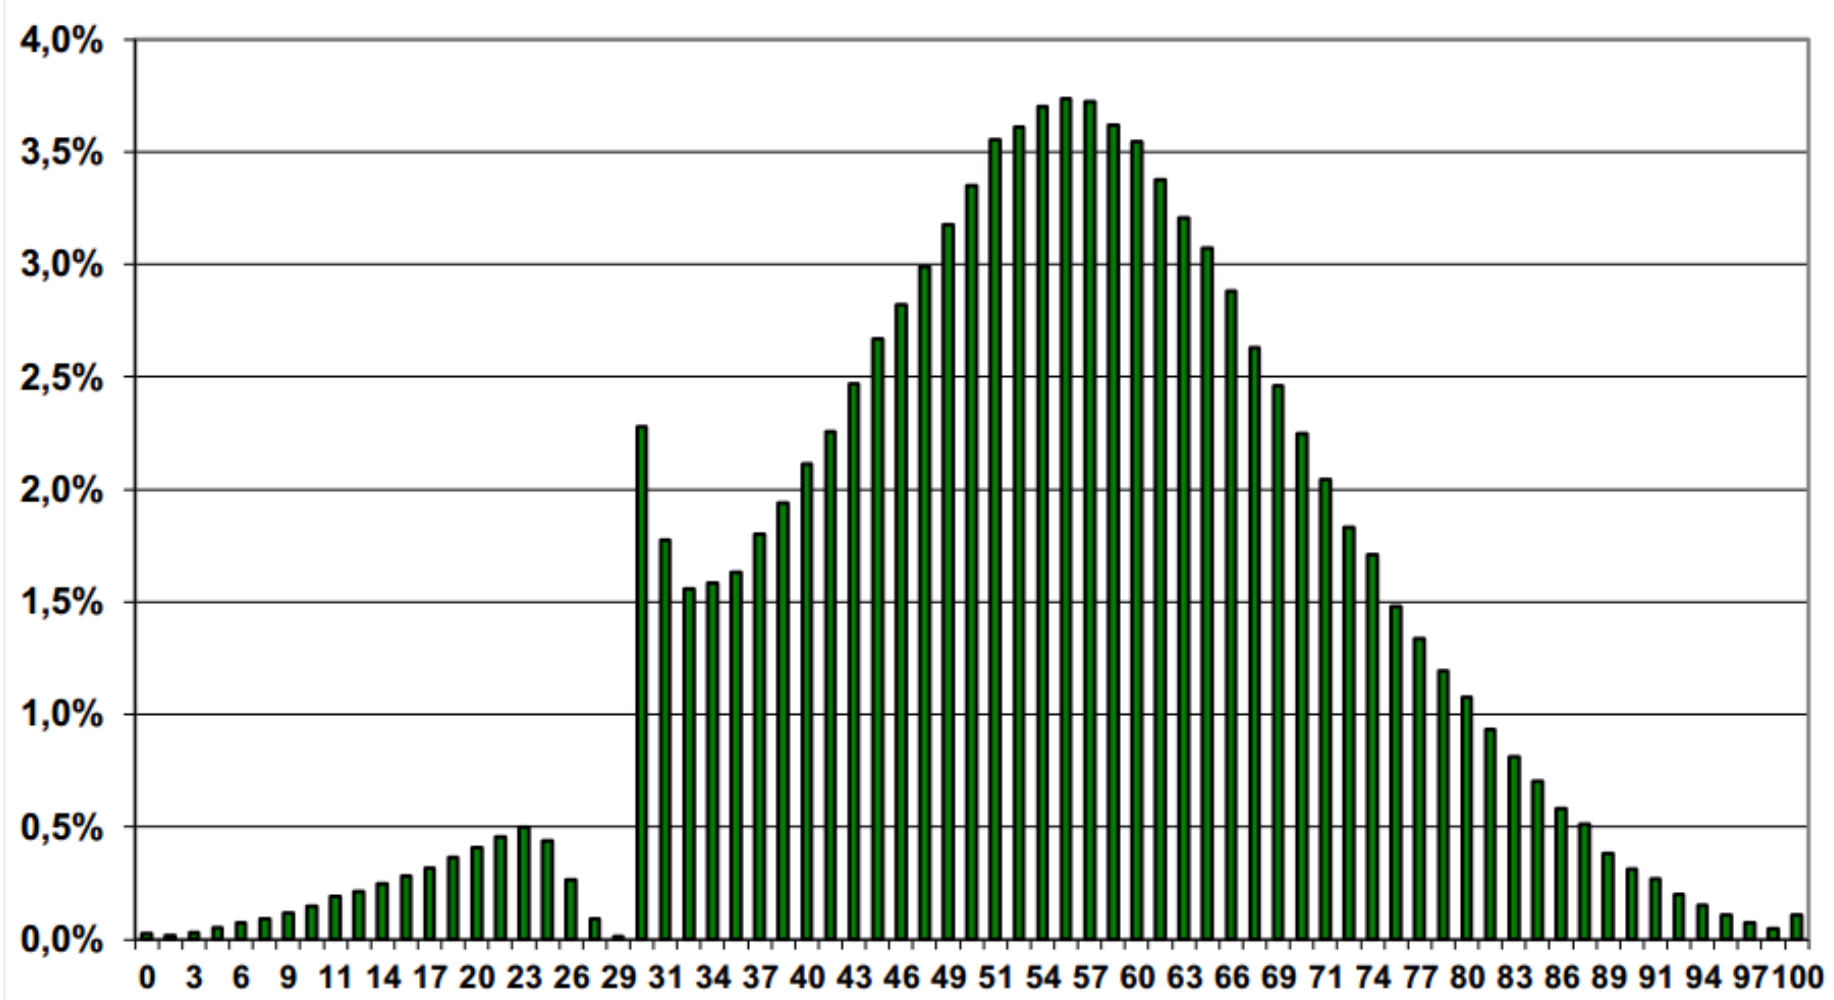
\includegraphics[width=0.7\linewidth]{poland_ege.png}
\end{center} 

Результаты экзаменов относятся к Средиземью. Довольно мало людей сдают их очень хорошо, довольно мало людей сдают их очень плохо. Чаще всего люди довольно старательные, и в среднем они довольно сильно похожи друг на друга. Поэтому распределение оценок за экзамен должно концентрироваться вокруг какого-то среднего. При этом хвосты распределения должны оказаться довольно тонкими. Другими словами говоря, результаты экзаменов укладываются в предпосылки ЦПТ и на выходе должны давать распределение, похожее на нормальное.

Понятное дело, что это всего лишь картинка. Сделать достоверные выводы по ней нельзя. Однако, если отталкиваться от такой логики, на гистограмме с распределением оценок можно заметить два артефакта. Во-первых, это подозрительный пик в районе $30$ баллов. Этот балл, скорее всего, был проходным. Этот пик явно искусственный. Скорее всего, проверяющие искусственно натянули результаты части людей, чтобы они не получили двойку. 

Во-вторых, можно заметить подозрительный маленький пик на $100$ баллах. Быть стобальником почётно. Возможно, что части $98-$ и $99-$бальников искусственно подарили этот почёт. Возможно, что этот пик приходится на олимпиадников, которым при победе в олимпиаде автоматически проставляется сто баллов. Возможно, что экзамен был слишком лёгким и на самом деле $100$ баллов было выставлено людям, которые были достойны $101, 102$ и т.д. баллов. Аналогичный второй горб мог бы возникнуть от $0$ до $20$ баллов, если бы всех студентов без разбора резко решили бы послать писать экзамен по китайскому языку. Однозначно можно сказать только то, что на гистограмме что-то не так. 

\subsection{Выборы выборы}

Явка на выборы, как случайная величина тоже укладывается в подобные предпосылки. Если попробовать строить гистограммы с явкой по разным избирательным участкам для Франции или Германии, то они внезапно оказываются колоколообразными.

В России на каждых выборах ЦПТ по какой-то причине отказывает\footnote{\url{https://clck.ru/Yws24}}. Правый хвост для правящей партии стабильно оказывается очень толстым. Более того, между величиной явки и долей голосов за неё есть положительная связь. Это выглядит довольно странно. Часть электоральных статистиков утверждает, что на выборах происходят фальсификации\footnote{\url{https://clck.ru/Yws4c}}. Центральная избирательная комиссия, в ответ на это, говорит, что Россия --- очень разнородная страна и из-за этого для случая сёл правый хвост оказывается завышен. В них обычно на выборы идут массово и поддерживают одну партию\footnote{\url{http://cikrf.ru/activity/relevant/detail/29380/}}. 

Электоральные статистики в ответ приводят пример Москвы, где на участках без комплексов автоматической обработки избирательных бюллетеней и наблюдателей, правый хвост завышен. При этом на участках, где это всё есть, кривая, описывающая явку куполообразная, а явка никак не коррелирует с числом голосов за какую-то партию. Подобные кривые строят по многим странам\footnote{\url{http://e-notabene.ru/pr/article_19136.html}}. Каких-то конкретных выводов по подобным гистограммам нельзя, но выглядят они крайне подозрительно.


\begin{thebibliography}{1}
% 	\bibitem{ref:chern}
% 	\emph{Н.И.Чернова} (2007).
% 	Теория вероятностей.~//
% 	\url{https://tvims.nsu.ru/chernova/tv/lec/node53.html}.
	
% 	\bibitem{ref:hanter}
% 	\emph{David Hunter} (2006).
% 	Asymptotic Tools.~//
% 	\url{http://personal.psu.edu/drh20/asymp/fall2006/lectures/}.	
	
% 	\bibitem{ref:pishro}
% 	\emph{H. Pishro-Nik} (2014).
% 	Introduction to probability, statistics, and random processes.~//
% 	\url{https://www.probabilitycourse.com}.	
	
	\bibitem{zhlobolite}
	\emph{Алексей Марков.}
	Жлобология.~//
	\url{https://alexeymarkov.ru/trial/zhlobolite.pdf}.
	
	\bibitem{ref:zmde}
	\emph{Howard Wainer} (2007).
	The Most Dangerous Equation.~//
	\url{http://nsmn1.uh.edu/dgraur/niv/TheMostDangerousEquation.pdf}.

	\bibitem{ref:pinker}
	\emph{Pinker, S.} (2011).
	The Better Angels of our Nature.~//
	\url{https://stevenpinker.com/publications/better-angels-our-nature}.	

	\bibitem{ref:taleb}
	\emph{Pasquale Cirillo, Nassim Taleb} (2015).
	On the statistical properties and tail risk of violent
conflicts~//
	\url{https://www.fooledbyrandomness.com/longpeace.pdf}.

	\bibitem{ref:quants}
	\emph{ } ( ).
	 ~//
	\url{ }.

	\bibitem{ref:gnedenko}
	\emph{ } ( ).
	 ~//
	\url{ }.



\end{thebibliography}

\end{document}


